\subsubsection{usergoal-ugLogin}

\label{RE-use-case-ugLogin}


An actor wants to identify himself in order to gain access to the systems functionalities		  


\begin{usecase}
  \addheading{Use-Case Description}
  \addsingletwocolumnrow{Name}{ugLogin}
  \addsingletwocolumnrow{Scope}{system}
  \addsingletwocolumnrow{Level}{usergoal}
  

\addrowheading{Primary actor(s)}
\addnumberedsinglerow{}{\msrcode{actAuthenticated[active]}}


\addrowheading{Secondary actor(s)}
\addnumberedsinglerow{}{\msrcode{actCaptchaGenerator[active]}}
\addnumberedsinglerow{}{\msrcode{actCaptchaValidator[active]}}
\addnumberedsinglerow{}{\msrcode{actMailingService[active]}}

\addrowheading{Goal(s) description}
\addsinglerow{An actor wants to identify himself in order to gain access to the systems functionalities}

\addrowheading{Reuse}
\addnumberedsinglerow{}{\msrucname{oeLogin [1..1]}}
\addnumberedsinglerow{}{\msrucname{oeSendCaptcha [1..1]}}
\addnumberedsinglerow{}{\msrucname{oeSubmitCaptcha [1..1]}}
\addnumberedsinglerow{}{\msrucname{oeCaptchaInvalid [1..1]}}
\addnumberedsinglerow{}{\msrucname{oeCaptchaValid [1..1]}}

\addrowheading{Protocol condition(s)}
\addnumberedsinglerow{}{the system has to be started}
\addnumberedsinglerow{}{the actor (client) must be able to access the system (connected to the internet)}

\addrowheading{Pre-condition(s)}
\addnumberedsinglerow{}{the actor is not identified (logged in) and thus not able to access the systems functionalities}

\addrowheading{Main post-condition(s)}
\addnumberedsinglerow{}{if the login was successful, the actor is now identified and thus able to access the systems functionalities}
\addnumberedsinglerow{}{if an attempt to log in failed, the authentication is refused and the actor has to try again}
\addnumberedsinglerow{}{if the actor failed three times to log in, each further attempt to log in is accompanied by a captcha verification test}
\addnumberedsinglerow{}{if the actor failed three times to log in without and five times with captcha verification, the requested user name will be blocked from further log in attempts}

\addrowheading{Main Steps}
\addalphanumberedsinglerow{}{the actor \msrcode{actAuthenticated} executes the \msrucname{oeLogin} use case}
\addalphanumberedsinglerow{}{the actor \msrcode{actCaptchaGenerator} executes the \msrucname{oeSendCaptcha} use case}
\addalphanumberedsinglerow{}{the actor \msrcode{actAuthenticated} executes the \msrucname{oeSubmitCaptcha} use case}
\addalphanumberedsinglerow{}{the actor \msrcode{actCaptchaValidator} executes the \msrucname{oeCaptchaInvalid} use case}
\addalphanumberedsinglerow{}{the actor \msrcode{actCaptchaValidator} executes the \msrucname{oeCaptchaValid} use case}
\addrowheading{Steps Ordering Constraints}
\addnumberedsinglerow{}{at least a}
\addnumberedsinglerow{}{if b then previously a}
\addnumberedsinglerow{}{if c then previously b}
\addnumberedsinglerow{}{if d then previously c}
\addnumberedsinglerow{}{if e then previously c}

\addrowheading{Additional Information}
\addsinglerow{
none
}

\end{usecase} 


Figure \ref{fig:lu.uni.lassy.excalibur.examples.icrash-RE-UCD-uc-ugLogin}
An actor tries to log in to the system using his credentials

\begin{figure}[htbp]
\begin{center}

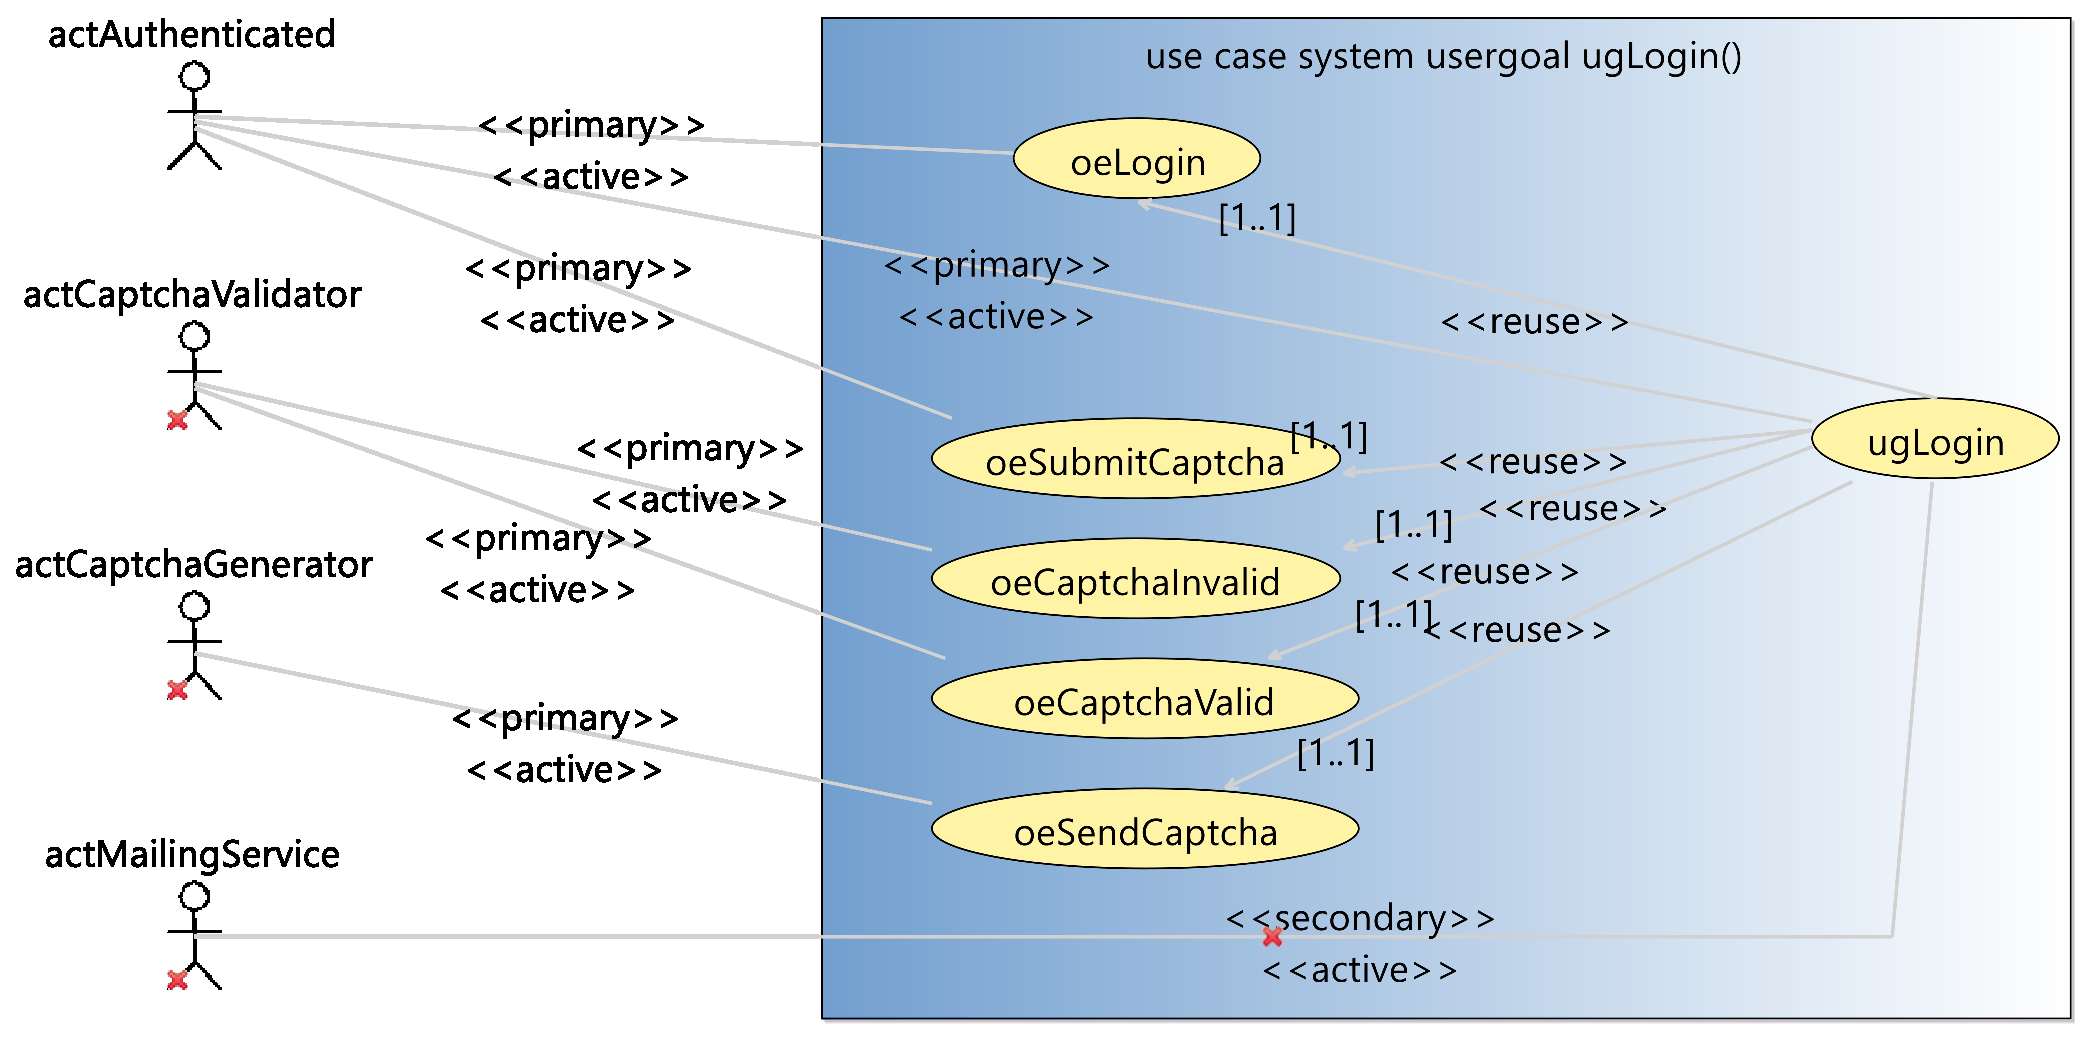
\includegraphics[
angle=0
,width=1.0\textwidth
]{./images-report-gen/usecase-model/usergoal/uc-ugLogin.eps}
\end{center}
\caption[lu.uni.lassy.excalibur.examples.icrash Use Case Diagram: uc-ugLogin]{User goal: log in to the system}
\label{fig:lu.uni.lassy.excalibur.examples.icrash-RE-UCD-uc-ugLogin}
\end{figure}
\vspace{0.5cm}
